\documentclass[a4paper,10pt]{article}

%A Few Useful Packages
\usepackage{marvosym}
\usepackage{fontspec} 					%for loading fonts
\usepackage{xunicode,xltxtra,url,parskip} 	%other packages for formatting
\usepackage{float}
\RequirePackage{color,graphicx}
\usepackage[usenames,dvipsnames]{xcolor}
\usepackage[big]{layaureo} 				%better formatting of the A4 page
% an alternative to Layaureo can be ** \usepackage{fullpage} **
\usepackage{supertabular} 				%for Grades
\usepackage{titlesec}					%custom \section

%Setup hyperref package, and colours for links
\usepackage{hyperref}
\definecolor{linkcolour}{rgb}{0,0.2,0.6}
\hypersetup{colorlinks,breaklinks,urlcolor=linkcolour, linkcolor=linkcolour}

%FONTS
\defaultfontfeatures{Mapping=tex-text}
%\setmainfont[SmallCapsFont = Fontin SmallCaps]{Fontin}
%%% modified for Karol Kozioł for ShareLaTeX use
\setmainfont[
SmallCapsFont = Fontin-SmallCaps.otf,
BoldFont = Fontin-Bold.otf,
ItalicFont = Fontin-Italic.otf
]
{Fontin.otf}
%%%

%CV Sections inspired by: 
%http://stefano.italians.nl/archives/26
\titleformat{\section}{\Large\scshape\raggedright}{}{0em}{}[\titlerule]
\titlespacing{\section}{0pt}{3pt}{3pt}
%Tweak a bit the top margin
%\addtolength{\voffset}{-1.3cm}

%Italian hyphenation for the word: ''corporations''
\hyphenation{im-pre-se}


%--------------------BEGIN DOCUMENT----------------------
\begin{document}

%WATERMARK TEST [**not part of a CV**]---------------
%\font\wm=''Baskerville:color=787878'' at 8pt
%\font\wmweb=''Baskerville:color=FF1493'' at 8pt
%{\wm 
%	\begin{textblock}{1}(0,0)
%		\rotatebox{-90}{\parbox{500mm}{
%			Typeset by Alessandro Plasmati with \XeTeX\  \today\ for 
%			{\wmweb \href{http://www.aleplasmati.comuv.com}{aleplasmati.comuv.com}}
%		}
%	}
%	\end{textblock}
%}

\pagestyle{empty} % non-numbered pages

\font\fb=''[cmr10]'' %for use with \LaTeX command

%--------------------TITLE-------------
\par{\centering
		{\Huge Xinyu \textsc{Jian}
	}\bigskip\par}

%--------------------SECTIONS-----------------------------------
%Section: Personal Data
\section{Personal Data}

\begin{tabular}{rl}
%    \textsc{Department:}& Naval Architecture and Ocean Engineering, Shanghai Jiao Tong University \\
    \textsc{Phone:}     & +86 13162080873 \\
    \textsc{email:}     & \href{mailto:heartwords368@gmail.com}{heartwords368@gmail.com}
\end{tabular}


%Section: Education
\section{Education}
\begin{tabular}{rl}	
  2015--2019 & \textbf{Shanghai Jiao Tong University (SJTU)}, Shanghai, China\\
  \\
 & \emph{B.S. in Naval Architecture and Ocean Engineering (major)}  \\
&\normalsize \textsc{Gpa}: 3.5/4.3 \hyperlink{grds}{\hfill | \footnotesize Detailed List of Exams}\\&\\
& \emph{B.S. in Mathmatics (minor)} \\
&\normalsize \textsc{Gpa}: \hyperlink{grds_cleli}{\hfill| \footnotesize Detailed List of Exams}\\&\\

\end{tabular}

\section{Research Experience}
\begin{tabular}{ll}

\textbf{The Research on the Communication and Control System of Wave Glider}& \\
\footnotesize{\emph{Researcher in State Key Laboratory of Ocean Engineering, SJTU (Advisor: A/Prof. Xinliang Tian)}} & \footnotesize{\hfill 2016--Now} \\
$\cdot$ \footnotesize{Design a simple communication system based on Iridium}& \\
$\cdot$ \footnotesize{Develop a simple on-board control system}&\\
$\cdot$ \footnotesize{H. Wang, Q. Cai, \textbf{X. Jian}, Z. Liu, P. Wang, X. Tian "Design of Communication and Control} \\\quad \footnotesize{System for the Wave Glider" \emph{Laboratory Research and Exploration} (In Preparation)}\\\multicolumn{2}{c}{} \\

\textbf{Experiment on the Piston and Slosh Motions of Moon Pools Under Exciting Force }&\\
\footnotesize{\emph{Researcher in the Towing Tank, SJTU (Advisor: Prof. Xinshu Zhang)}} & \footnotesize{\hfill 2017--Now} \\
$\cdot$ \footnotesize{Design the experiment model} & \\
$\cdot$ \footnotesize{Design the method to collect the data} & \\\multicolumn{2}{c}{} \\

\textbf{The Research on the Obstacle Detection of Unmanned Sailboat}&\\
\footnotesize{\emph{Researcher in Unmanned Sailboat Club, SJTU (Advisor: A/Prof. Jinsong Xu)}}& \footnotesize{\hfill Now}\\
$\cdot$ \footnotesize{Responsible for the obstacle detection}
\end{tabular}


\section{Skills}
\begin{tabular}{rl}
 Programming language:& Python, \textsc{C++}, Java, \textsc{MATLAB}, \textsc{html5}, \textsc{css} \\
 Professional software:& AutoCAD, SolidWorks, Patran/Nastran\\
 MCU:& STM32, Arduino, Raspberry\\
Others:&{\fb \LaTeX}, Linux, Netlogo, $\mu$Vision\\
\end{tabular}


%Section: Scholarships and additional info
\section{Scholarships and Certificates}
\begin{tabular}{lcl}
National Endeavor Scholarship & \href{http://www.moe.gov.cn/jyb_xwfb/xw_zt/moe_357/jyzt_2015nztzl/2015_zt06/15zt06_gxzzzc/gxzz_bzks/201508/t20150810_199203.html}{Link}& 2016,2017\\
Cyrus Tang Scholarship & \href{http://www.tangfoundation.org/index.php?option=com_content&view=article&id=12&Itemid=89&site=CTF&sub=0}{Link}& 2016,2017 \\ 
SDARI Scholarship &  & 2017 \\
1\textsuperscript{st} Prize in National Marine Vehicle Competition & \href{http://www.csname.org.cn/qghyhxqds/325112.htm}{Link} & 2017
\end{tabular}

%Section: Language
\section{Language}
\begin{figure}[H]
    \centering
    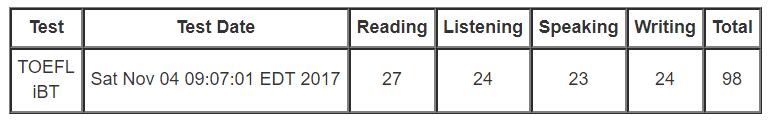
\includegraphics{TOEFL.PNG}
\end{figure}


\newpage
\par{\centering\Large \hypertarget{grds}{Master of Science in \textsc{Finance}}\par}\large{\centering Grades\par}\normalsize
\begin{center}
\begin{tabular}{lcc}
\multicolumn{1}{c}{\textsc{Exam}}&\textsc{Grade}&\textsc{Credit Hrs}\\ \hline
Corporate Finance (Valuation)	&25&	6\\
Financial Statement Analysis	&28&	6\\
Statistics	&27&	6\\
Theory of Finance	&26&	6\\
Quantitative Methods for Finance	&30&	6\\
Econometrics	&24	&6\\
Derivatives	&31&	6\\
Management of Financial and Insurance Companies	&30&	6\\
Business Law	&31&	6\\
Investment Banking	&28&	6\\ \\
		
Behavioral Models for Economics and Finance	&29&	6\\
Numerical Methods for Finance	&29&	6\\
Advanced Derivatives	&30&	6\\
Fixed Income (Advanced Methods)	&30&	6\\ \\
		
English Language	&30&	4\\
French Language	&31&	4\\
		
Internship	&	&8\\
		
Final Thesis	&	&20\\
		
		& Total&120\\\cline{2-3}
&\textsc{Gpa}&\textbf{28.61}
\end{tabular}
\end{center}
\bigskip
\hrule
\bigskip
\par{\centering\Large \hypertarget{grds_cleli}{Undergraduate Degree in \textsc{Law and Business Administration}}\par}\large{\centering Grades\par}\normalsize

\begin{center}

\tablefirsthead{%
  \multicolumn{1}{c}{\textsc{Esame (\textsc{ita})}}&\multicolumn{1}{c}{\textsc{Exam (\textsc{eng})}}&\textsc{Grade}&\textsc{Credit Hrs}\\ \hline}
\tablehead{%
\multicolumn{1}{c}{\textsc{Esame (\textsc{ita})}}&\multicolumn{1}{c}{\textsc{Exam (\textsc{eng})}}&\textsc{Grade}&\textsc{Credit Hrs}\\ \hline
}
\tabletail{%
}
\tablelasttail{}	

 \begin{supertabular}{p{4.9cm} p{4.9cm} c c}
Economia aziendale&Theory and principles of management& 28 & 8\\
Istituzioni di diritto privato&Principles of private law&30&8\\
 Istituzioni di diritto pubblico 
&
 Principles of public law 
& 30&
 6 
\\
Matematica generale 
& Mathematics 
&31&8\\
 Contabilit\`a e Bilancio 
& Accounting and Financial statements 
& 31 & 8\\
 Diritto del lavoro 
&
 Labour law 
& 30&
4 
\\
 Informatica & Computer skills &29& 4 
\\
 Economia e gestione delle imprese & Corporate management &31&6 
\\
 Microeconomia & Microeconomics &30&8 
\\
 Contabilit\`a e bilancio 2 & Accounting and financial statements 2 
&29&8 \\
 Diritto commerciale & Company and business law &30&8 
\\
 Macroeconomia & Macroeconomics &29&8 
\\
 Statistica & Statistics &30&6\\
 Diritto delle procedure concorsuali & Insolvency law &31&4 
\\
 Finanza aziendale 
& Corporate finance 
&31 &8 \\
 Matematica finanziaria & Financial mathematics &31&4 
\\
 Programmazione e controllo 
& Management accounting &31&8 
\\
Lingua Inglese \textsc{c1}& English Language \textsc{c1}& 25&6\\ 
Diritto tributario & Tax law &30&6 
\\
Organizzazione e sistemi informativi aziendali &Management information systems &28&6 
\\
 Strategia e politica aziendale* 
& Business strategy* & 29& 6 
\\
Derivati*&Derivatives*&30&6\\
Opzionale all'estero* & Corporate Financial Strategy* &30&6\\
Lingua Francese \textsc{b1} & French Language \textsc{b1}&31&6\\
Economia dei mercati e degli intermediari finanziari* 
&Financial markets and institutions* &30&6 
\\
Revisione aziendale 
&Financial auditing &31&6 
\\
Scienza delle finanze &Public economics &30&6 
\\
 Lavoro finale& Final report&&6\\
& & Total&180\\\cline{3-4}
& &\textsc{Gpa}&\textbf{29.85}\\ \\ \multicolumn{4}{l}{\footnotesize A star (*) indicates that the course was taken at the \textbf{University of Southern California}, Los Angeles, \textsc{usa}}
 \end{supertabular}
\end{center}
\bigskip
\hrule
\bigskip
\par{\centering\Large \hypertarget{grds_usc}{Exchange Program at \textsc{usc}, Los Angeles}\par}\large{\centering Grades\par}\normalsize

\begin{center}
\begin{tabular}{lcc}
\multicolumn{1}{c}{\textsc{Exam}}&\textsc{Grade}&\textsc{Grade Points}\\ \hline
Corporate Financial Strategy	&A&	4\\
Derivatives	&A&	4\\
Money, Credit, and Banking	&A&	4\\
Business Strategy & A-& 3.5\\
& &\\\cline{2-3}
 &\textsc{Gpa}&\textbf{3.875}
\end{tabular}
\end{center}
%\newpage
%\hypertarget{gmat}{\textsc{Gmat}\setmainfont{LMRoman10 Regular}\textregistered\setmainfont[SmallCapsFont=Fontin-SmallCaps]{Fontin-Regular}}

%\XeTeXpdffile ''GMAT.pdf'' page 1 scaled 800

\end{document}
